\section{Theory}
\label{chap:theory}
\subsection{The Transmission electron microscope}
The Transmission electron microscope (TEM) is a microscope that far exceeds the capabilities of a normal light microscope. Both types of microscope use a series of lenses to magnify the image of a specimen.
A normal light microscope can amplify an image up to about 1500$\times$ and is limited by the diffraction limit. Assuming an average wavelength of 550$nm$ for green light a high-end microscope is limited to resolving features 100$nm$ apart.
This limit is too low for looking at atomic structures.\cite{PhysRevLett.106.193905}\\
An electron microscope circumvents this limit by using electrons, not light, to probe the specimen. Electrons when accelerated have a smaller wavelength than light thus allowing for images with resolved features as small as 0.05$nm$. \cite{kisielowski_freitag_bischoff_van}
The TEM works by releasing electrons from an electron source and accelerating them to an energy typically expressed in kilo-electronvolt. After being accelerated the electrons pass multiple electromagnetic lenses and a condenser aperture to shape the beam before it 'illuminates' the specimen as illustrated in \ref{fig:tem}.
The beam incident on the sample is limited to a illumination semi-angle $\alpha$ which is inversely proportional to the resolution, but limiting $\alpha$ decreases the amount of electrons incident on the specimen and thus a frame needs more time for a decent exposure.
After having interacted with the specimen the beam is again limited by an aperture, this aperture sets the collection semi-angle $\beta$ which controls the limit of scattering angles allowed into the imaging lenses.
After the beam is conditioned by the imaging lenses it passes trough four electromagnetic prisms which make up an energy filter called an $\Omega$-filter named after the shape it needs to have to keep the TEM stack aligned with the CCD-camera to limit aberrations.
The $\Omega$-filter is used for energy filtered TEM images discussed in section \ref{sec:eftem}.\\
Two types of images can be made with the TEM, a normal image which shows the magnified sample and a diffraction pattern image which can be made by placing the capture device in the focal point of the lens and filter system.
A diffraction mode image shows the diffraction peaks that are characteristic of the sample and yields information on the reciprocal lattice of the sample. \cite{Egerton_2008}


%+ Normal microscope
%+ Electron microscope resolution
%+ Workings with diagram
%+ Imaging modes


\begin{figure}
	\centering
	
\includegraphics[width=0.25\linewidth, keepaspectratio]{tem.png}
	\caption{TEM}
	\label{fig:tem}
\end{figure}

\subsection{Crystal structure}
A crystal is build up of unit cells in such a way that the whole crystal can be made by shifting and aligning unit cells. These unit cells are build up of atoms whose position in the unit cell can be fully expressed in terms of primitive basis vectors. If the crystal were to be cut in half by a plane this plane would be expressed by fractional coordinates, these fractional coordinates show where along a basis vector the plane and basis vector intersect. Such a plane is called a Miller plane and the corresponding coordinates are called the Miller indices. Miller planes that have the same orientation but are shifted to different unit cells share the same Miller indices and are called a family of planes. The crystal structure of $\gamma$-IndiumSelenide with its basis vectors and unit cell is shown in figure \ref{fig:inse}.
In reciprocal space the diffraction spots correspond to a certain family of planes, the position of diffraction spots can be expressed in reciprocal basis vectors. A reciprocal basis unit cell is shown in figure \ref{fig:unit-cell}. In this figure the high-symmetry directions are also shown as arrows.

\begin{minipage}{0.5\textwidth}
	\centering
	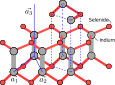
\includegraphics[width=0.45\linewidth, keepaspectratio]{inse.png}
	\captionof{figure}{inse}
	\label{fig:inse}
\end{minipage}%
\begin{minipage}{0.5\textwidth}
	\centering
	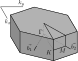
\includegraphics[width=0.45\linewidth, keepaspectratio]{unit-cell.png}
	\captionof{figure}{unit}
	\label{fig:unit-cell}
\end{minipage}

\subsection{Electron scattering theory}
In a TEM setup electrons are essentially shot through a sample in which the electrons can either simply pass through or scatter, in the latter scenario there are two possibilities, electrons can scatter elastically or inelastically.
Scattering is a result of the interaction between the sampling electrons from the TEM source and the charges particles in the specimen.\\
When scattering elastically the electrons interact with a nucleus of the specimen whose mass is many times greater than that of the sampling electron, resulting in a small and usually unmeasurable energy transfer.
In a crystalline specimen electrons can only be scattered at certain angles due to the crystal structure creating a diffraction pattern of bright spots. In cases of large scattering angles the electron does transfer a significant amount of energy and can even reverse direction, this energy transfer can permanently displace atoms in the crystal structure causing a defect.\\
When the sampling electron interacts with an electron in the specimen's crystal lattice inelastic occurs due tot the similarity in mass between the two electrons. The energy transfer of this interaction ranges from a few electronvolts up to multiple hundreds of electronvolts.
Inelastic scattering not only results in an energy transfer but also in a momentum transfer as shown in figure \ref{fig:scat}, the $k'$-vector shows a scattered electron that deviates from the not scattered electron vector $k_0$.
The total momentum transfer is the sum of the perpendicular momentum transfer $q_{\perp}$ proportional to the scattering angle $\theta$ and the momentum transfer parallel to the undisturbed path due to an energy transfer from the sampling electron to the sample. This parallel momentum transfer is thus proportional to the energy loss of the electron.
Figure \ref{fig:bands} shows the band structure of the crystalline sample of which the electrons scatter. In this figure two bands are shown, both bands can be occupied by electrons of certain energies, to excite an electron from the blue band to the red band an electron needs either energy (path $t_1$) or energy and momentum (path $t_2$).
The needed energy and momentum are transferred from an incident sampling electron in the inelastic interaction. By measuring the energy and momentum of a scattered electron it is possible to piece together all the combinations of energy and momenta transfer possible and thus find the band structure of the sample.\\
Another form of inelastic scattering is plasmon excitation.\\
Since the outer-shell electrons of an atom are only weakly bound to the nucleus due to screening effects but are coupled together by electrostatic interaction. These delocalised electrons form an energy band similar to that shown in figure \ref{fig:bands}.
When a fast-moving sampling electron is shot through the sample all nearby outer-shell electrons are displaced. If the sampling electron's velocity exceeds the fermi speed the displacement of outer-shell electrons creates an oscillating ripple creating waves of alternating positive and negative electric charge, this is known as a plasmon wake.



\begin{figure}
	\centering
	\includegraphics[width=0.25\linewidth, keepaspectratio]{scat.png}
	\caption{The elastic scattering $k'$ of an electron over an angle $\theta$ due to the interaction with a crystalline sample.}
	\label{fig:scat}
\end{figure}

\begin{figure}
	\centering
	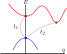
\includegraphics[width=0.25\linewidth, keepaspectratio]{bands.png}
	\caption{The band structure of the crystalline sample in fig. \ref{fig:scat} showing both a direct bandgap $t_1$ and an indirect bandgap $t_2$.}
	\label{fig:bands}
\end{figure}


\subsection{Momentum resolved electron energy-loss spectroscopy}
\label{sec:MREELS}
Momentum resolved electron energy-loss spectroscopy hereafter abbreviated as MREELS is a TEM imaging technique in which the imaging plane of the CCD camera is placed in the focal point of the imaging lenses and energy filter.
This allows the camera to take a diffraction mode image in which the diffraction pattern of the scattering electrons is shown. This is illustrated in figure \ref{fig:diff-im}. In this figure the crystalline sample is shown as the box with the slanted lines that represent the Miller planes of the crystal structure.
As shown in the figure all electrons that scatter of of the same family of Miller planes get focused on the same region on the imaging sensor, electrons that do not scatter also get focused in one spot at the centre of the diffraction pattern.
A diffraction mode image does not image normal space but instead shows reciprocal space which is also the reason this type of image is useful. In a normal image one would attribute lengths to the axes of an image but in a diffraction mode image the separation of features is given by a momentum difference.
The separation of the light and dark grey arrows on the imaging plane in figure \ref{fig:diff-im} is thus equal to the difference in perpendicular momentum transfer between scattering electrons (light grey) and electrons that do not scatter (dark grey).
Since the momentum transfer for the electrons that do not scatter is zero the momentum transfer for scattering of a certain family of planes can be determined.


\begin{figure}
	\centering
	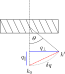
\includegraphics[width=0.25\linewidth, keepaspectratio]{diff-im.png}
	\caption{scat}
	\label{fig:diff-im}
\end{figure}
\begin{figure}
	\centering
	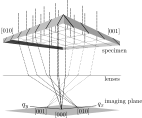
\includegraphics[width=0.75\linewidth, keepaspectratio]{diff-im3d.png}
	\caption{scat}
	\label{fig:diff-im3d}
\end{figure}





\subsubsection{Energy filtered transmission electron microscope}
\label{sec:eftem}
An energy filtered transmission electron microscope is a microscope with an energy filter placed in the optical column of the TEM. Energy filtering is accomplished by the use of electromagnetic prisms such as those shown in figure \ref{fig:filter}.
These prisms just like ordinary prism disperse the electrons with different wavelengths proportional to electron energy. By sliding a slit into the cone of dispersed electrons it is possible to choose a finite range of electron energies to image.
The EFTEM setup can be used in conjunction with the MREELS imaging technique to gather information on both the momentum transfer of the electron (via MREELS) and the energy loss associated (via EFTEM) with that momentum transfer.

\begin{figure}
	\centering
	
\includegraphics[width=0.25\linewidth, keepaspectratio]{filter.png}
	\caption{A $\Omega$-spectrometer spreading the electrons based on their energy and a slit selecting energies to focus on the CCD camera.}
	\label{fig:filter}
\end{figure}

\subsection{Diffraction image}
In a diffraction mode image there are a set of bright spots in momentum space for which scattering probability is high. These bright spots correspond to a family of planes, to determine to which family of planes the bright spots correspond they first have to be indexed. Indexing is done by using the geometric properties of the image to narrow down how the image is oriented.
By measuring the distance from the middle brightest spot to one of the closer outward ones, measuring the angle between lines connecting these spots and searching for these values in a database it is possible to determine to zone and orientation of the image \footnote{A huge thank you to A. Brokkelkamp for showing how to index the diffraction image}. Once the image is indexed the family of planes can be attributed to the bright diffraction spots as done in figure \ref{fig:tr-diff-im}.

\begin{figure}
	\centering
	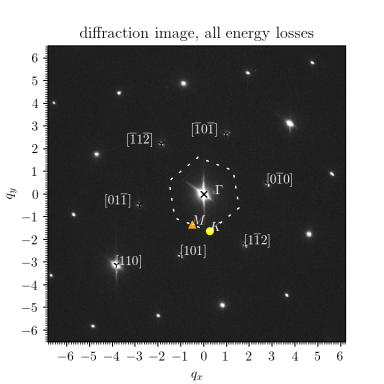
\includegraphics[width=0.5\linewidth, keepaspectratio]{tr-diff-im.png}
	\caption{A diffraction mode image showing the total scattering intensity at momentum space positions. The diffraction spots are indexed with Miller indices. The $M$- and $K$-point and first Brillouin zone are also shown.}
	\label{fig:tr-diff-im}
\end{figure}



\subsection{q-EELS spectra and q-EELS map}
An electron energy loss spectroscopy spectrum is a plot that show the scattering intensity at a certain energy loss $\Delta E$ of the electron, a q-EELS spectrum also has a momentum transfer value $q_{\perp}$ that corresponds to the whole spectrum. A q-EELS spectrum is plotted in figure \ref{fig:spectrum}, this spectrum corresponds to a momentum transfer of zero and is thus in the middle of the centre diffraction spot. The spectrum starts with a high peak in the low-loss region, this peak is called the zero-loss peak and shows the high intensity of electrons not losing energy and in this case momentum when passing trough the sample. This peak is a problem since it masks the interesting low-loss data completely.\\
The q-EELS map shows the same energy loss spectra but for multiple momenta transfers at a time. For every combination of energy loss and momentum transfer there is a single intensity value which is shown in colour, the brighter the pixel the more electrons scatter with that combination of energy loss and momentum transfer. A q-EELS map is pictured in figure \ref{fig:qmap}, the zero-loss peaks still show as the bright streak at $0 \Delta eV$ for all momenta transfers. This spectrum was created by walking the path from $\Gamma$ to $M$ and then to $K$ in which the points are the same as in figure \ref{fig:tr-diff-im}.

\begin{minipage}{.45\textwidth}
	\centering
	\captionsetup{width=0.8\linewidth}
	\includegraphics[width=1.0\linewidth, keepaspectratio]{big-spectrum.eps}
	\captionof{figure}{EELS spectrum of $\gamma$-InSe for $q_{\perp}=0$}
	\label{fig:spectrum}
\end{minipage}%
\begin{minipage}{.45\textwidth}
	\centering
	\captionsetup{width=0.8\linewidth}
	\includegraphics[width=1.0\linewidth, keepaspectratio]{qmap-example.eps}
	\captionof{figure}{q-EELS map of $\gamma$-InSe along $\Gamma \rightarrow M \rightarrow K$}
	\label{fig:qmap}
\end{minipage}

\subsection{Physical relevance of (MR)EELS data}
As hinted at in section \ref{sec:MREELS}, the combination of both energy and momentum information allows for the reconstruction of the band structure of the specimen. This information can be used to determine the density of states of the specimen \cite{doi:10.1021/acs.nanolett.9b03928} \cite{Egerton_2008}.
EELS spectra can also be used to determine the electronic properties of the specimen, the bandgap of a semiconductor and the dielectric function, as well as mechanical properties \cite{Egerton_2008}.
Different signature peaks in the EELS data can be used to determine the elemental makeup of the specimen \cite{Egerton_2008}.